% The \phantomsection command is needed to create a link to a place in the document that is not a
% figure, equation, table, section, section, chapter, etc.
%
% When do I need to invoke \phantomsection?
% https://tex.stackexchange.com/questions/44088/when-do-i-need-to-invoke-phantomsection
\phantomsection


% Multiple-language document - babel - selectlanguage vs begin/end{otherlanguage}
% https://tex.stackexchange.com/questions/36526/multiple-language-document-babel-selectlanguage-vs-begin-endotherlanguage

\chapter[Experiments]{Experimental Evaluation}\label{sec:experiments}

\begin{flushright}
     
\end{flushright}

To evaluate the proposed measure we performed three different experiments. The two first experiments use real and well known trajectory datasets: the taxi trajectories in San Francisco from the CRAWDAD project \cite{epfl-mobility-20090224} and the Geolife dataset \cite{zheng2009mining}. The third experiment uses a synthetic trajectory dataset, created using the Hermoupolis \cite{Pelekis-Hermoupolis} trajectory generator, which generates semantic trajectories with \emph{stops} and \emph{moves}. In the Geolife and taxi datasets we evaluate the similarity of both stops and moves, where the \emph{moves} similarity is evaluated considering its raw points, while in the synthetic dataset we consider several types of semantic information associated to the \emph{moves}. 

We also evaluated how SMSM is impacted by changing its parameters and compare the running time of SMSM and the other similarity measures, for both raw and semantic trajectories.

We evaluate the precision of SMSM by the retrieval-based approach (\textit{precision at recall}), computing the Area Under the Curve (AUC) and Mean Average Precision (MAP). To calculate the precision at recall, the trajectories are segregated into \textit{T\textsubscript{class}} by their classes and were used as the ground truth trajectories. For each ground truth trajectory, the $|$\textit{T\textsubscript{class}}$|$ most similar trajectories should also belong to \textit{T\textsubscript{class}}. For each one, a similarity search over the dataset is performed, ranking the trajectories until all \textit{T\textsubscript{class}} trajectories are found. Ideally, a similarity measure should return all trajectories in the ground truth between 1 to $|$\textit{T\textsubscript{class}}$|$ positions. The results of precision at each recall level are the average obtained for all \textit{T\textsubscript{class}} trajectories at that recall level. {We compared SMSM with the following state-of-the-art similarity measures: MSM, LCSS, EDR, MSTP, CVTI, DTWa, wDF, and UMS.}

Section \ref{sec:new_crawdad} describes the experiment with the {taxi} dataset, Section \ref{sec:geolife} details the experiments with the Geolife dataset, Section \ref{sec:hermoupolis} details the experiments with the synthetic dataset, Section {\ref{sec:sensitivity}} details the experiments changing the SMSM parameters, Section {\ref{sec:running_time}} evaluates the running time of the similarity measures, and Section {\ref{sec:discussion}} presents a discussion about the choice of a measure in face of application problems.

\section{Experiment with the taxi dataset}\label{sec:new_crawdad}

The epfl/mobility dataset contains taxi trips in San Francisco collected between May and June 2008, with an average sampling rate of about one point per minute. Each trajectory has several days of duration, what is not useful to determine similar movements around the town. For that reason, we split each taxi trajectory into short trajectories, (i) splitting when the occupation status of the taxi changed (taken or free) and (ii) splitting when a 5 minutes gap between two consecutive points was found\hl{, because if a taxi is 5 minutes not sending any GPS signal is expected the car is off.}

\subsection{Ground truth generation}
{In this experiment we defined six distinct regions in San Francisco with high density of trajectories moving between these regions, which are shown in Figure {\ref{fig:new_sanfrancisco_map_rois}}(left). The regions are the \textbf{Park}, the \textbf{Fisherman's Wharf}, the \textbf{Pier}, the Westfield San Francisco Center (\textbf{WSFC}), the \textbf{Intersection} between highways 280 and 101, and San Francisco \textbf{Airport}. In total, there are 6940 trajectories moving between these regions.}

\begin{figure}[ht!]
\centering
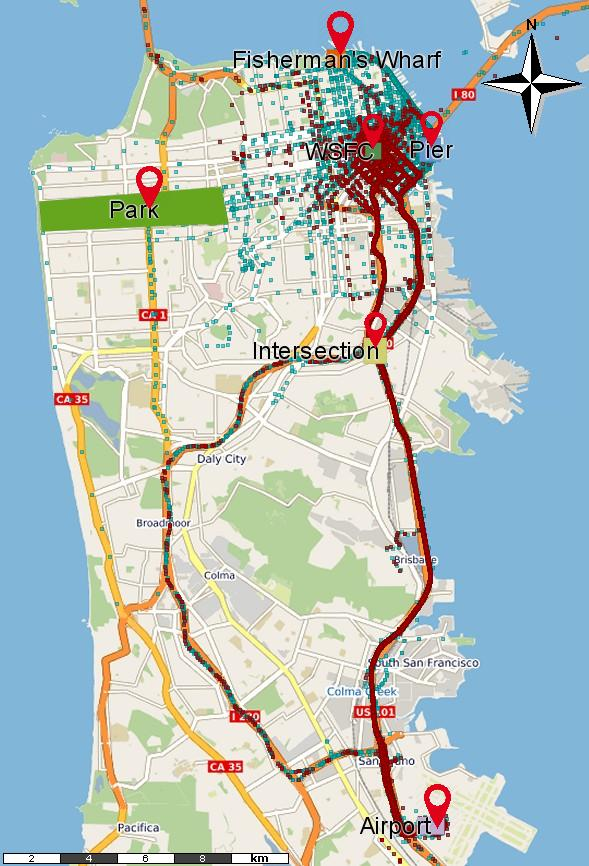
\includegraphics[width=.45\textwidth]{Images/new_CRAWDAD-Trajectories-Painted}
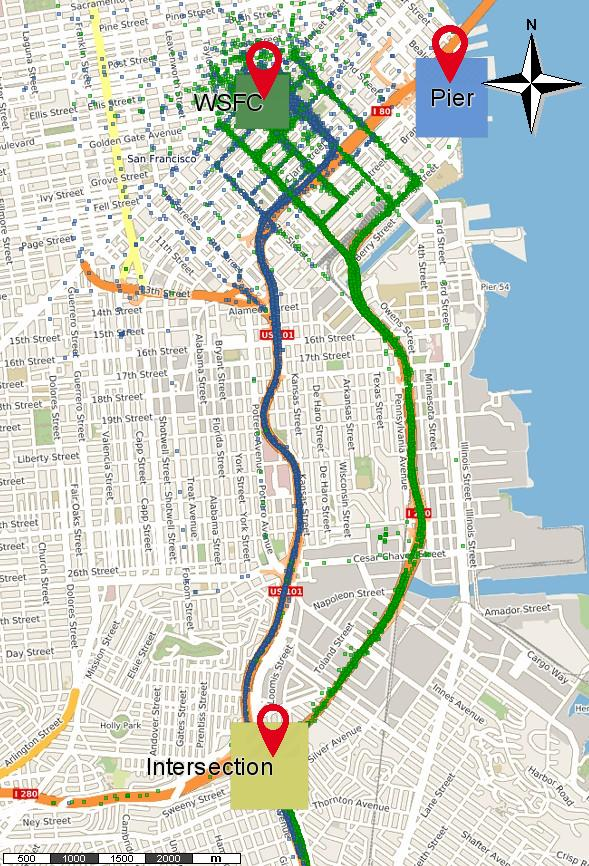
\includegraphics[width=.45\textwidth]{Images/new_CRAWDAD-Paths-Painted}
\caption{(left) All trajectories moving between the six regions, where the red points are the ground truth trajectories and the light blue points are the remaining trajectories. (right) Ground truth trajectories, where dark blue points are the trajectories moving on highway 101 and green points are trajectories using highway 280}
\label{fig:new_sanfrancisco_map_rois}
\end{figure}

As ground truth we consider the subset of trajectories moving between Airport,  Intersection, and WSFC. These trajectories were selected because they have different moves.  Figure {\ref{fig:new_sanfrancisco_map_rois}} (right) shows a zoom over the trajectories moving between  \textbf{Airport} and \textbf{WSFC}  using the \textbf{Intersection} of highways 101 (blue) and 280 (green), where we can visualize that the trajectories have different \emph{moves}. We consider as the ground truth the four distinct paths followed by the trajectories that move between these regions, which are shown in Table {\ref{tab:new_san_francisco_dataset}}. There are 145 trajectories moving from Airport in direction to WSFC via highway 101, which we define as class A1. There are 1242 trajectories moving in the opposite direction, from WSFC to the Airport by highway 101, that are labeled as class A2. There are 531 trajectories moving from Airport in direction to WSFC by highway 280, which we label as class B1, and 704 trajectories moving from WSFC in direction to Airport by highway 280, which are labeled as class B2. We assume that trajectories that belong to the same class should be more similar than trajectories of different classes.

\begin{table}[h]
\scriptsize
  \centering
  \begin{tabular}{|c|c|c|c|c|}
  \hline
 Direction & Highway & Trajectories & Class \\
  \hline
 Airport to WSFC & 101 & 145 & A1\\
 WSFC to Airport & 101 & 1242 & A2\\
 Airport to WSFC & 280 & 531 & B1\\
 WSFC to Airport & 280 & 704 & B2\\
    \hline
  \end{tabular}
  \caption{Ground truth trajectories}
  \label{tab:new_san_francisco_dataset}
\end{table}

\subsection{Results for the taxi trajectories}

In this experiment we considered the following dimensions for stops and moves: as spatial dimension of the stops we considered the centroid of the stop; as temporal dimension we used both start and end time of the stop; and as semantic information we used the name of the region (WSFC, Pier, Fisherman's Wharf, Park, Intersection, and Airport). For the moves we analyze the real movement, and use as spatial dimension the moves raw points.

For measuring the stop similarity we use: (i) the Euclidean distance for space; (ii)  distance 0 in case of exact match for semantics and 1 otherwise; and (iii) for the time dimension, where $[t1, t2]$ is the time interval of a stop, the time distance of two stops is given by  Equation {\ref{func:time_interval}}. For the moves, we consider the raw trajectory points and use the UMS measure for the move spatial similarity, because it is the most appropriate for low sampled trajectories, which is the case for this dataset.

In this experiment we consider the same weights for each dimension and for stops and moves, so 0.5 for the stops and 0.5 for the moves, and 0.33 for the dimensions space, time, and semantics. Later in the parameter analysis section we show how the results change as we vary the weights of the stops and moves, as they are the central contribution of this thesis.

As several measures were not developed for semantic trajectories, for a more fair comparison we apply existing measures over semantic trajectories and over raw trajectories. For doing so we split the experiment in two parts: 1) a \textit{precision at recall} evaluation using only semantic trajectories; and 2) a \textit{precision at recall} evaluation using the raw trajectories.

Table \ref{tab:new_san_francisco_measures} summarizes the dimensions used in each measure. To general multidimensional similarity measures as MSM, we provide as input all dimensions of each stop, namely: 1) spatial information; 2) time interval; and 3) semantic information. We extend LCSS and EDR to support multiple dimensions: given two multidimensional trajectories, two points match when all dimensions match, where each dimension has a distinct distance threshold. With those adaptations, both LCSS and EDR are used to measure similarity using the dimensions of space, time and semantics for stops. For CVTI, we provide as input the time interval of the stops and the stop names. For MSTP, we provide the stop names only.

\begin{table}[!h]
\scriptsize
  \centering
  \begin{tabular}{|l|c|c|c|c|c|}
  \hline
  & \multicolumn{4}{c|}{Semantic trajectories} & \multicolumn{1}{c|}{Raw trajectories} \\
 	\cline{2-5}
  & \multicolumn{3}{c|}{Stop} & \multicolumn{1}{c|}{Move} & \multicolumn{1}{c|}{} \\
 	\cline{2-6}
  & Space & Time & Semantics & Trajectory points & Space\\
  \hline
 SMSM & \checkmark & \checkmark & \checkmark & \checkmark & \\
 MSM & \checkmark & \checkmark & \checkmark & &\\
 MSTP &  &  & \checkmark & & \\
 CVTI & & \checkmark & \checkmark & & \\
 LCSS & \checkmark & \checkmark & \checkmark & & \checkmark \\
 EDR & \checkmark & \checkmark & \checkmark & & \checkmark \\
 DTWa &  &  &  & & \checkmark \\
 UMS & & & & & \checkmark \\
 wDF & & & & & \checkmark \\
    \hline
  \end{tabular}
  \caption{Dimensions used for each measure}
  \label{tab:new_san_francisco_measures}
\end{table}

{Table {\ref{tab:new_san_francisco_thresholds}} shows the  thresholds used for each measure. To define threshold values for the stops we experimented  a range of values on each dimension as follows: for space (distance between stop centroids) we varied the distance from 100 meters to 500 meters in a 100 meters range; and for the time distance we tested a proportion of intersection from 0\% to 100\% varying in ranges of 10 \%. For the move threshold we varied the UMS similarity for two moves from 0 to 1 in a 0.1 unit step.

Table {\ref{tab:new_sanfrancisco_measures_map_auc}} shows the comparison of SMSM with approaches developed either for raw or semantic trajectories.
For semantic trajectories, SMSM (MAP=0.84) outperformed the other measures in 50\% or more. This occurs because state-of-the-art measures do not take into account the move between two stops or consider only stops. We may notice that the second best measure for semantic trajectories is MSM, but it reaches only 39\% of precision. This shows that MSM is not robust when considering both stop and move similarity, because MSM cannot deal with moves and does not distinguish the order of the stops, i.e., the direction of the trajectories. 
For raw trajectories, SMSM (MAP=0.84) was 27 \% better than UMS (MAP=0.62) and DTWa (MAP=0.61), that were the most accurate measures apart from SMSM. Both UMS and DTWa perform worse than SMSM because on the contrary to MSM, they consider only raw trajectories, and cannot deal with stops and their semantics.}

\begin{table}[!h]
\scriptsize
  \centering
  \begin{tabular}{|c|c|c|c|c|}
  \hline
  & \multicolumn{3}{c|}{Semantic trajectories} & \multicolumn{1}{c|}{Raw trajectories} \\
 	\cline{2-5}
  & Space (meters) & Time proportion & Move & Space (meters) \\
  \hline
 SMSM & 100 & 0.3 & 0.8 & - \\
 MSM & 100 & 0.1 & - & - \\
 LCSS & 100 & 0.1 & - & 100 \\
 EDR & 100 & 0.1 & - & 100 \\
    \hline
  \end{tabular}
  \caption{Thresholds used for each measure}
  \label{tab:new_san_francisco_thresholds}
\end{table}


\begin{table}[h]
\scriptsize
  \centering
  \begin{tabular}{|l|c|c|c|c|}
  \hline
 & \multicolumn{2}{c}{Semantic} & \multicolumn{2}{|c|}{Raw} \\
 	\cline{2-5}
 & MAP & AUC & MAP & AUC \\
  \hline
SMSM & \textbf{0.84} & \textbf{0.87} & - & -\\
UMS & - & - & 0.62 & 0.66 \\
DTWa & - & - & 0.61 & 0.65 \\
wDF & - & - & 0.47 & 0.51 \\
MSM & 0.39 & 0.42 & - & - \\
EDR & 0.26 & 0.30 & 0.36 & 0.40 \\
LCSS & 0.29 & 0.33 & 0.34 & 0.38 \\
MSTP & 0.30 & 0.33 & - & - \\
CVTI & 0.28 & 0.32 & - & - \\
    \hline
  \end{tabular}
  \caption{MAP and AUC evaluation for the taxi dataset}
  \label{tab:new_sanfrancisco_measures_map_auc}
\end{table}


Figure \ref{fig:new_sanfrancisco_precision_recall} (left) and Figure \ref{fig:new_sanfrancisco_precision_recall} (right) {summarize the results of \emph{precision at recall}  of all similarity measures. On the left, SMSM was better to recover trajectories of the same class than the other methods in almost all recall levels, being around  60\% more precise than  state-of-the-art measures. On the right, we may notice that the measures developed for raw trajectories performed well, because the trajectories of the different classes are partially discriminated by the moves, characterized by the trajectory raw points. These measures do not perform better because they ignore the semantic dimensions and the stops.}


\begin{figure*}[ht!]
\centering
\centerline{
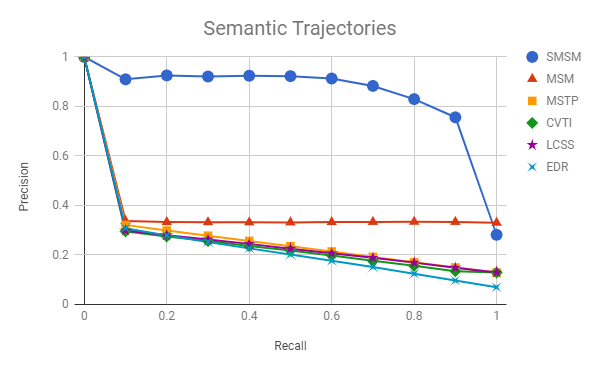
\includegraphics[width=0.5\textwidth]{Images/new_P_R-chart_San_Francisco.png}
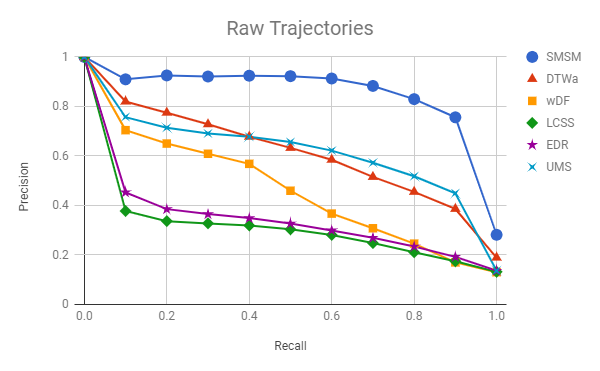
\includegraphics[width=0.5\textwidth]{Images/new_P_R-chart_San_Francisco-raw.png}
}
\caption{ Precision at recall results for semantic and raw trajectories}
\label{fig:new_sanfrancisco_precision_recall}
\end{figure*}


\section{Experiment with the Geolife Dataset}\label{sec:geolife}

The Geolife is a well-known trajectory dataset, created by Microsoft Research Asia \cite{zheng2009mining} containing trajectories of 182 users, moving around Beijing, collected between April 2007 and August 2012. As a preprocessing step, we split trajectories when a 5 minutes gap between two consecutive points was found, since the trajectories of this dataset are highly sampled (lower than 2s).

\begin{figure}[ht!]
\centering
\centerline{
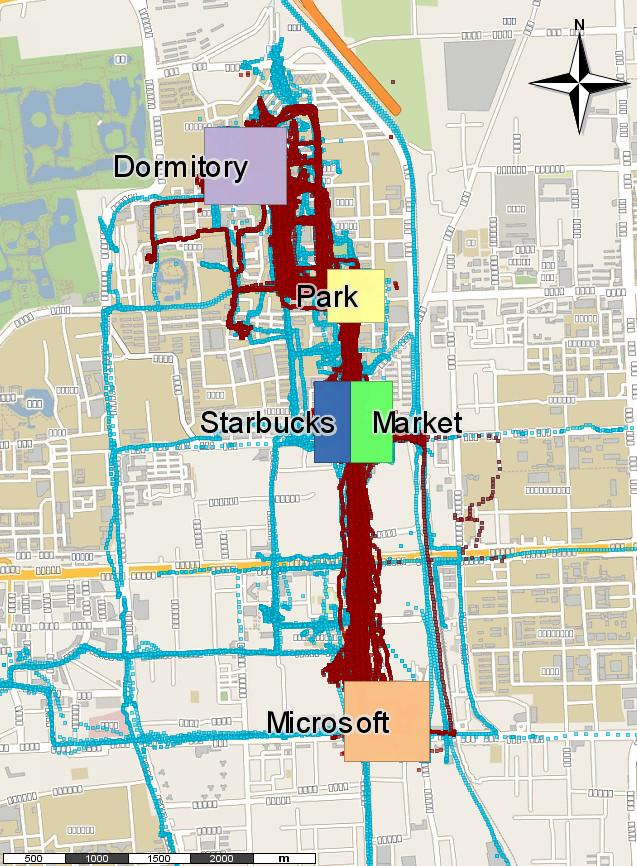
\includegraphics[width=.5\textwidth]{Images/new_Geolife-Trajectories-painted.jpg}
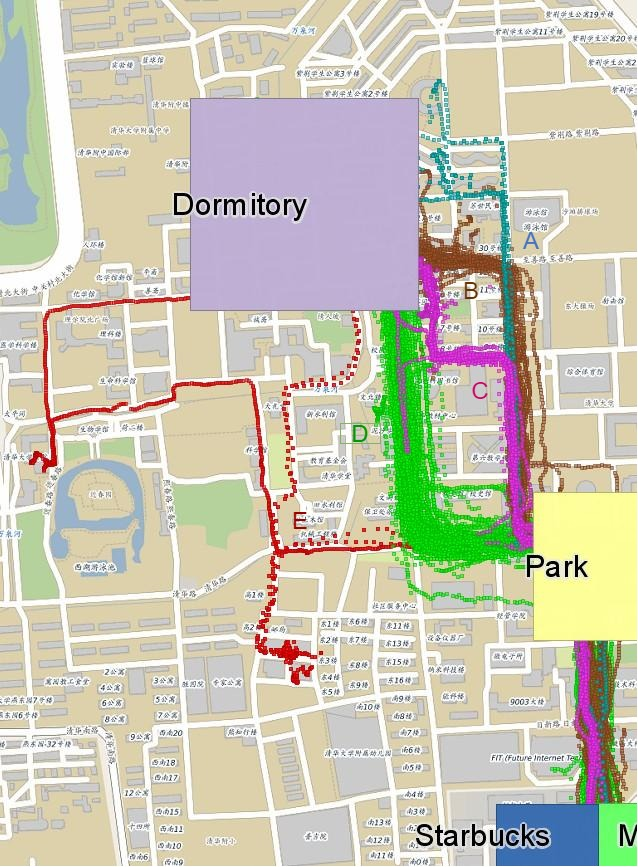
\includegraphics[width=.5\textwidth]{Images/Geolife-Paths-painted.jpg}
}
\caption{(left) All trajectories moving between the five regions, where the red points are the ground truth trajectories and the light blue points are the remaining trajectories. (right) zoom over the ground truth trajectories moving between Park and Dormitory to observe their moves}
\label{fig:geolife_map_rois}
\end{figure}


\subsection{Ground Truth Definition}
{As in the previous experiment, the Geolife dataset has no ground truth for evaluating similarity measures, so we had to generate a ground truth. We had to find stops where the objects make different moves between the stops in order to distinguish the trajectories.}
To build the ground truth, we chose an area in Beijing, where pedestrians move between the University Dormitories and Microsoft Research Office. We considered five places as stops (Microsoft, Starbucks, Market, Park and Dormitory), that are shown in Figure \ref{fig:geolife_map_rois} (left). {We selected $1976$ trajectories that pass over two or more of these places. Among the $1976$ trajectories we defined as ground truth the $337$ trajectories that go from Microsoft to Dormitory (and vice versa) passing by Park and Market or Starbucks.} We considered 5 distinct paths connecting the stops, labeled as A, B, C, D, and E, as shown in Figure \ref{fig:geolife_map_rois} (right).

In Table \ref{tab:geolife_dataset} we define as ground truth 8 distinct classes of movement based on the sequence of stops and the followed path: Microsoft to Dormitory via Market and Park by path A with 5 trajectories named as class A, Microsoft to Dormitory via Market and Park by path B with 40 trajectories named as class B, Dormitory to Microsoft via Park and Starbucks by path C with 11 trajectories named as class C, Dormitory to Microsoft via Park and Starbucks by path D with 115 trajectories named as class D1, Dormitory to Microsoft via Park and Market by path D with 7 trajectories named as class D2, Microsoft to Dormitory via Market and Park by path D with 149 trajectories named as class D3, Microsoft to Dormitory via Starbucks and Park by path D with 6 trajectories named as class D4 and Microsoft to Dormitory via Market and Park by path E with 4 trajectories named as class E.

It is worth mentioning that in this experiment, similar to the previous one, the moves are characterized by the raw trajectory points and we use these points to compare stops and moves similarity.

\begin{table}[ht!]
\scriptsize
  \centering
  \begin{tabular}{|c|c|c|c|}
  \hline
 Direction & Path &  Trajectories & Class \\
  \hline
Microsoft to Dormitory via Market and Park& A & 5 & A \\
Microsoft to Dormitory via Market and Park& B & 40&B \\
Dormitory to Microsoft via Park and Starbucks& C & 11&C \\
Dormitory to Microsoft via Park and Starbucks& D & 115&D1 \\
Dormitory to Microsoft via Park and Market& D & 7&D2 \\
Microsoft to Dormitory via Market and Park& D & 149&D3 \\
Microsoft to Dormitory via Starbucks and Park& D & 6&D4 \\
Microsoft to Dormitory via Market and Park& E & 4& E \\
    \hline
  \end{tabular}
  \caption{Classes representing distinct paths of the ground truth}
  \label{tab:geolife_dataset}
\end{table}

\subsection{Results with the Geolife dataset}

Following a similar methodology used for the previous experiment, we calculate the precision at recall for all classes in the ground truth (8), comparing the SMSM results to the other measures. The dimensions used for stops are: a) space; and b) the region name (Dormitory, Park, Starbucks, Market and Microsoft). For the moves we used the raw points of the move. The time dimension was not taken into account because in this experiment there are classes with a few trajectories and most of them do not match in time.

For measuring the stop similarity we use: (i) the Euclidean distance for space; and (ii) 1 and 0 for the semantics in case of exact match or no match, respectively. For the moves,  we consider the raw trajectory points. In this experiment we use DTW distance for analyzing the spatial similarity of the moves, because the trajectory points are highly sampled {and trajectory points are very near in space}.
For this dataset UMS is not the best measure for distinguishing the moves, since it was developed for irregular sampling. \hl{When the points are highly sampled, UMS tends to build small ellipses, so giving low similarity degree for very similar/close trajectories}. For the weights we give the same importance for stops and moves, so we use 0.5 for stops and 0.5 for moves and for the dimensions, we use 0.5 for space and 0.5 for semantics.

Table \ref{tab:geolife_thresholds} presents the thresholds used for each measure. We defined the thresholds by running each experiment over a range of possible threshold values and the best results for each method are reported. For raw trajectories, we evaluated as threshold the  values 2, 4, 6, 8 and 10 meters because this dataset is highly sampled and is of pedestrian trajectories. The threshold for the move dimension was defined as follows: two moves are said to match if the DTW distance between them is less than the sum of the Euclidean distance of the moves. \hl{We used this approach for the move comparison because the DTW distance of two points sequence is not a bounded value as UMS, which score the similarity between 0 and 1, but an unbounded value.}

\begin{table}[!h]
\scriptsize
  \centering
  \begin{tabular}{|c|c|c|}
  \hline
  & \multicolumn{1}{c|}{Semantic trajectories} & \multicolumn{1}{c|}{Raw trajectories} \\
 	\cline{2-3}
  & Space (meters) & Space (meters) \\
  \hline
 SMSM & 100 & - \\
 MSM & 100 & - \\
 LCSS & 100 & 8 \\
 EDR & 100 & 8 \\
    \hline
  \end{tabular}
  \caption{Thresholds used for each measure}
  \label{tab:geolife_thresholds}
\end{table}

Table \ref{tab:geolife_measures_map_auc} shows the experimental results.  {SMSM (MAP=0.94) outperforms all measures for semantic trajectories, being significantly better than MSM (MAP=0.66), which ignores the moves and the sequence of stops, so it is not able to distinguish trajectories that move in the opposite direction. On the other hand, EDR (MAP=0.72) performs better than MSM because it considers the sequence, and the order of the stops distinguishes the classes. The measures for raw trajectories perform very well because of the low number of stops in this dataset and because the raw trajectories are similar in terms of space, and the classes were build based on the moves spatial similarity, so benefiting DTWa (MAP=0.92), LCSS (MAP=0.81), and EDR (MAP=0.81). }


\begin{table}[ht!]
  \scriptsize
  \centering
  \begin{tabular}{|l|c|c|c|c|}
  \hline
 & \multicolumn{2}{c}{Semantic trajectories}& \multicolumn{2}{|c|}{Raw trajectories}\\
 	\cline{2-5}
 & MAP & AUC & MAP & AUC\\
  	\hline
SMSM & \textbf{0.94} & \textbf{0.95} & - & -\\
DTWa & - & - & 0.92 & 0.93\\
 EDR & 0.72 & 0.73 & 0.81 & 0.83\\
LCSS & 0.27 & 0.30 & 0.81 & 0.83\\
 UMS & - & - & 0.70 & 0.73\\
 MSM & 0.66 & 0.68 & - & -\\
 wDF & - & - & 0.54 & 0.58\\
CVTI & 0.30 & 0.34 & - & -\\
MSTP & 0.28 & 0.32 & - & -\\
    \hline
  \end{tabular}
  \caption{MAP and AUC evaluation for the experiment with the Geolife dataset}
  \label{tab:geolife_measures_map_auc}
\end{table}


\begin{comment}
\begin{table}[ht!]
  \scriptsize
  \centering
  \begin{tabular}{|l|c|c|c|c|}
  \hline
 & \multicolumn{2}{c}{Semantic}& \multicolumn{2}{|c|}{Raw}\\
 	\cline{2-5}
 & MAP & AUC & MAP & AUC\\
  \hline
SMSM & \textbf{0.95} & \textbf{0.96} & - & -\\
DTWa & - & - & 0.93 & 0.94\\
LCSS & 0.74 & 0.75 & 0.82 & 0.84\\
 EDR & 0.74 & 0.75 & 0.81 & 0.84\\
 UMS & - & - & 0.70 & 0.73\\
 MSM & 0.69 & 0.71 & - & -\\
 wDF & - & - & 0.58 & 0.61\\
CVTI & 0.43 & 0.46 & - & -\\
MSTP & 0.41 & 0.44 & - & -\\
    \hline
  \end{tabular}
  \caption{MAP and AUC evaluation for the experiment with the Geolife dataset}
  \label{tab:old_geolife_measures_map_auc}
\end{table}
\end{comment}

{Figure {\ref{fig:geolife_precision_recall}} shows the precision at recall results. Figure {\ref{fig:geolife_precision_recall}} (left) shows that SMSM was better to recover semantic trajectories of the same class in all recall levels, while Figure {\ref{fig:geolife_precision_recall}} (right) shows that all measures developed for raw trajectories, except wDF, performed well, but  the closest results to SMSM were achieved with DTWa.}


\begin{figure*}[ht!]
\centerline{
\centering
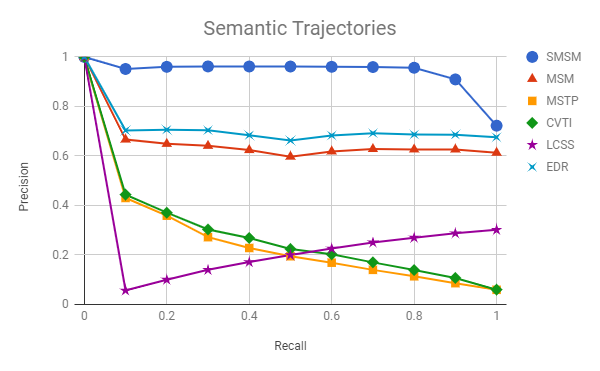
\includegraphics[width=.55\textwidth]{Images/new_P_R-chart_Geolife.png}
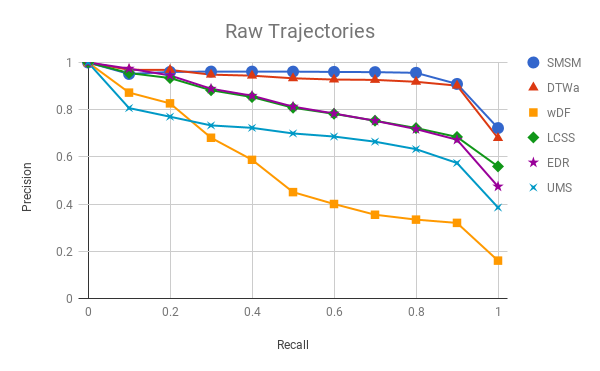
\includegraphics[width=.55\textwidth]{Images/new_P_R-chart_Geolife-raw.png}
}
\caption{Precision at recall results to semantic (left) and raw (right) trajectories}
\label{fig:geolife_precision_recall}
\end{figure*}

\section{Evaluation with a synthetic Dataset}\label{sec:hermoupolis}
The objective of this experiment with synthetic data is to evaluate trajectory similarity considering trajectories with different number of stops and the semantic dimensions of the moves, instead of the raw points of the move that were evaluated in the previous experiments.

We generate the trajectories with the  Hermoupolis trajectory generator \cite{Pelekis-Hermoupolis}, that allows creating trajectories based on pre-defined profiles. It generates semantic trajectories where both \emph{stops} and \emph{moves} are semantically enriched with annotations defined by the user. Therefore, it is possible to enrich the \emph{moves} between the \emph{stops} with semantic information, such as the transportation mean, the goal of the \emph{move}, the name of the streets, etc. Hermoupolis has several parameters to simulate real trajectories, such as the definition of the average time of the moving object at each \emph{stop}, the standard deviation of the time of each \emph{stop}, the speed of the moves, sampling rate, and so on. We generated 440 trajectories with several stops and moves, using as semantics of the \emph{stops} the POI category and the activity performed at the \emph{stop}. For the moves we generated the raw points with the following attributes:(i) the transportation mode; (ii) the activity performed during the \emph{move}; (iii) the traveled distance; (iv) the average speed; and (v) the duration of the move.

{There are two main differences of this experiment in relation to the previous ones: (i) the trajectories of the ground truth have a different number of stops and (ii) the moves have several and heterogeneous dimensions.}

\subsection{Ground Truth Definition}
{In this experiment we defined two classes, summarized in Table {\ref{tab:hermoupolis_dataset}}: (i) students with a job (80 trajectories); and (ii) students without a job (60 trajectories). What distinguishes the classes in this experiment is not the followed paths, but mainly the time and the duration  of the stops, as well as the transportation mode and the activity performed during the move. Besides the 140 trajectories of the ground truth, we generated 300 other trajectories in the same area, with distinct behaviors, to make the retrieval task more challenging.}

\begin{table}[ht!]
\scriptsize
  \centering
  \begin{tabular}{|c|c|c|}
  \hline
  Class & Trajectories & number of stops \\
  \hline
Student worker & 80 & 4 and 5 \\
Only student & 60 & between 4 and 7 \\
    \hline
  \end{tabular}
  \caption{Ground truth trajectories}
  \label{tab:hermoupolis_dataset}
\end{table}

{Figure {\ref{fig:hermoupolis_groundtruth}} (left) shows the generated trajectories, where the points in blue are the trajectories of the ground truth, while the brown points represent the remaining trajectories of the dataset. Some stops are Home, University, Supermarket, Restaurant, Bar, Mall, etc.
Figure {\ref{fig:hermoupolis_groundtruth}} (right) shows the trajectories of the ground truth.}

\begin{figure*}[ht!]
\centerline{
\centering
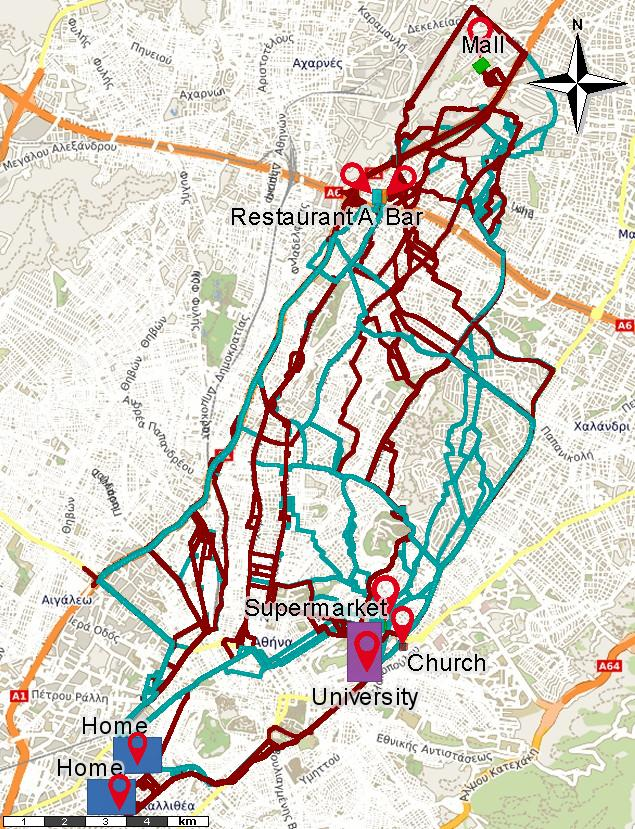
\includegraphics[width=.5\textwidth]{Images/Hermoupolis-RawPoints.jpg}
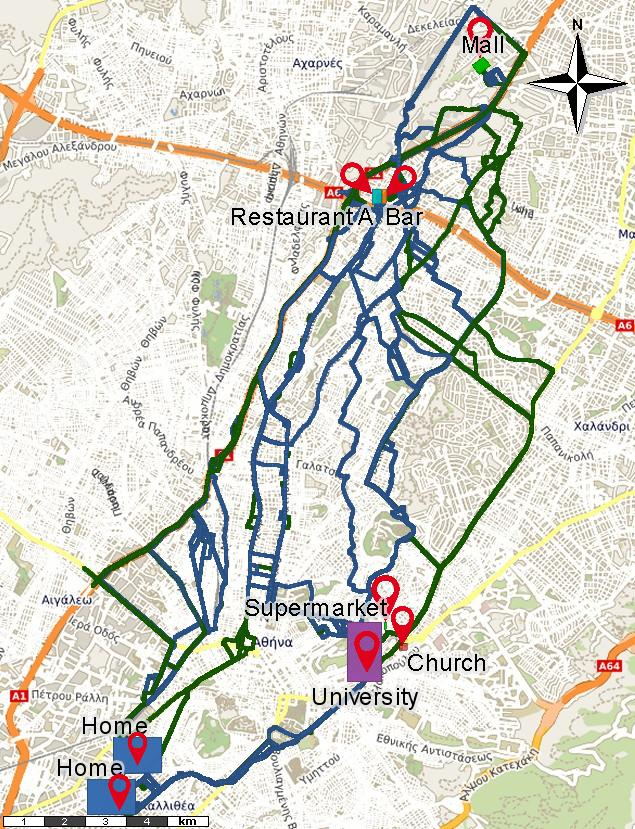
\includegraphics[width=.5\textwidth]{Images/Hermoupolis-CommercialCenter.jpg}
}
\caption{(left) Hermoupolis generated trajectories in red (ground truth) and light blue (remaining) and (right) Ground truth trajectories in green (student worker) and blue (only student).}
\label{fig:hermoupolis_groundtruth}
\end{figure*}

\subsection{Results with the Synthetic Dataset}
{Following the methodology used in the previous experiments, we calculate the precision at recall for the two classes in the ground truth, comparing the results of SMSM with the other measures. The dimensions used for the \emph{stops} are: a) the spatial centroid of the \emph{stop}; b) the duration of the \emph{stop}; and c) the \emph{stop} name (Home, Mall, University, etc). For the \emph{moves} we used several dimensions, including  the transportation mode, the activity performed during the move, the traveled distance, average speed, and duration.}

{For measuring the \emph{stops} similarity, we use: (i) the Euclidean distance for space; (ii) the proportion of the intersection between the time intervals of two \emph{stops}, as given by Equation {\ref{func:time_interval}}; and (iii) 1 for the semantics in case of exact match and 0 for no match. For the \emph{moves}, the transportation mode and activity have  similarity as 1 in the case of exact match and 0 otherwise. The weights for the \emph{stops} and the \emph{moves} are the same ($0.5$), and $0.33$ for of the  dimensions space, time, and semantics. The thresholds used for each measure are shown in Table {\ref{tab:hermoupolis_thresholds}}.  As in the previous experiments, we define the thresholds for each dimension after having tested a range of values in each dimension (space and time), and the best results are reported for each measure.}

\begin{table}[!h]
\scriptsize
  \centering
  \begin{tabular}{|c|c|c|c|}
  \hline
  & \multicolumn{2}{c|}{Semantic trajectories} & \multicolumn{1}{c|}{Raw trajectories} \\
 	\cline{2-4}
  & Space (meters)& Time (intersection proportion) & Space (meters) \\
  \hline
 SMSM & 300 & 0.1 & - \\
 MSM & 300 & 0.2 & - \\
 LCSS & 100 & 0.2 & 8 \\
 EDR & 100 & 0.2 & 8 \\
    \hline
  \end{tabular}
  \caption{Spatial and temporal thresholds used for each measure}
  \label{tab:hermoupolis_thresholds}
\end{table}

{Table {\ref{tab:hermoupolis_measures_map_auc}} presents the experimental results, in which we tested SMSM with several  attributes over the moves, and the best results where achieved with the dimensions transportation mode and activity. Comparing with measures for semantic trajectories, SMSM (MAP=0.95) was around 14\% more precise than LCSS (MAP=0.82), EDR (MAP=0.82) and MSM (MAP=0.81). The other measures for semantic trajectories had worse results, with MAP scores of 0.40 and 0.33 for MSTP and CVTI, respectively. As can be noticed in the results,  SMSM did not perform well for the dimensions duration, average speed, and traveled distance, because these dimensions are extracted from the moves raw points. As this experiment is characterized by the semantic dimensions of the moves, we can also notice that the measures for raw trajectories (EDR (MAP=0.51), DTWa (MAP=0.45), LCSS (MAP=0.44), UMS (MAP=0.29)) that performed well in the previous dataset where the moves raw points were considered, achieved at maximum 51\% of precision in the current experiment.}


\begin{table}[h]
\scriptsize
  \centering
  \begin{tabular}{|l|c|c|c|c|}
  \hline
 & \multicolumn{2}{c}{Semantic} & \multicolumn{2}{|c|}{Raw} \\
 	\cline{2-5}
 & MAP & AUC & MAP & AUC \\
  \hline
SMSM (Transportation Mode)& \textbf{0.95} & \textbf{0.95} & - & -\\
SMSM (Activity)& \textbf{0.93} & \textbf{0.94} & - & -\\
SMSM (Duration)& 0.73 & 0.75 & - & -\\
SMSM (Average Speed)& 0.72 & 0.75 & - & -\\
SMSM (Traveled Distance)& 0.72 & 0.74 & - & -\\
EDR & 0.82 & 0.85 & 0.51 & 0.54 \\
LCSS & 0.82 & 0.85 & 0.44 & 0.47 \\
MSM & 0.81 & 0.83 & - & - \\
DTWa & - & - & 0.45 & 0.48 \\
MSTP & 0.40 & 0.44 & - & - \\
wDF & - & - & 0.35 & 0.39 \\
CVTI & 0.33 & 0.37 & - & - \\
UMS & - & - & 0.29 & 0.33 \\
    \hline
  \end{tabular}
  \caption{MAP and AUC evaluation for the Hermoupolis dataset}
  \label{tab:hermoupolis_measures_map_auc}
\end{table}

{Figure {\ref{fig:hermoupolis_precision_recall}} (left) shows the precision at recall curves for all similarity measures developed for semantic trajectories. SMSM, using the transportation mode as the semantic dimension of the moves, is more accurate at each level, but EDR, LCSS, and MSM had   good results despite considering only the stops. All the remaining measures present worse results. Figure {\ref{fig:hermoupolis_precision_recall}} (right) shows the precision at recall curves for similarity measures developed for raw trajectories.  In this dataset, all similarity measures developed for raw trajectories had poor results, because each class has several paths for each move, but what distinguishes the moves are not the raw points, but the transportation mode.}

\begin{figure*}[ht!]
\centerline{
\centering
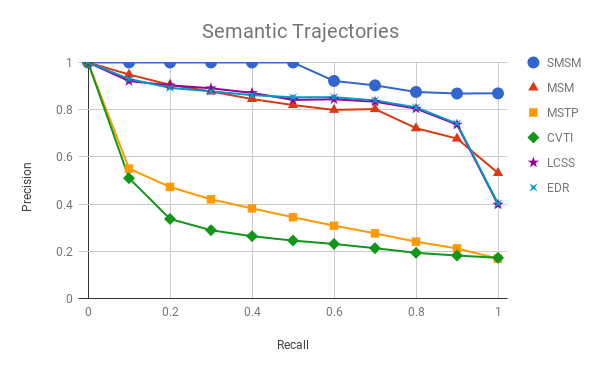
\includegraphics[width=.45\textwidth]{Images/P_R-chart_Hermoupolis_semantic.png}
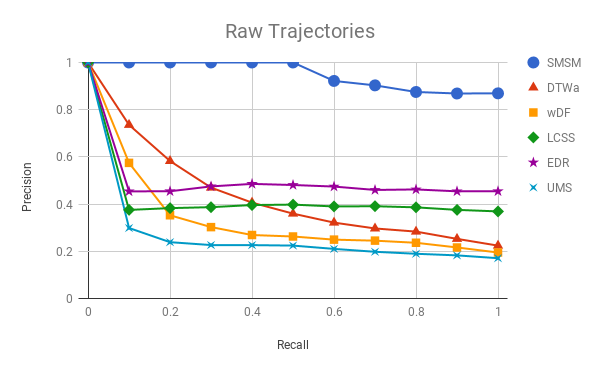
\includegraphics[width=.45\textwidth]{Images/P_R-chart_Hermoupolis_raw.png}
}
\caption{(left) Precision at recall results for semantic trajectories  and (right) Precision at recall results for raw  trajectories}
\label{fig:hermoupolis_precision_recall}
\end{figure*}


\section{Parameter Analysis}\label{sec:sensitivity}

{SMSM has two important groups of parameters: i) the \emph{weights} to define the importance of stops/moves and dimensions; and ii) the spatial \emph{threshold} to define if two stops match in order to analyze the moves.
With the weights framework, SMSM is flexible to give more or less importance to the stops, moves, and dimensions. 
}

To show the impact of the weight parameters on the similarity analysis, we evaluate the \emph{weight} of the \emph{stops} and the \emph{moves} in all experimental datasets. Table {\ref{tab:sensibility_stopmove}} shows the results for the weight varying from 0 to 1, where 0 means that the moves will be ignored and 1 means that only the moves will be considered.  As can be seen, if the influence of the \emph{moves} is ignored, i.e., weight = 0, and all importance is given to the stops, SMSM reaches a MAP score of only $0.49$ in the Taxi dataset, $0.72$ in the Geolife dataset, and $0.75$ in the synthetic dataset, indicating a confusion between the similarity of the trajectories that are also discriminated by the moves. The best average result is achieved when the weight of the \emph{moves} is set as 0.5, i.e, half of the weight goes for the stops and the other half to the moves.

\begin{table}[ht!]
  \scriptsize
  \centering
 \resizebox{\linewidth}{!}{%
  \begin{tabular}{|c|c|c|c|c|}
  \hline
Stop weight & Move weight & Taxi (MAP) & Geolife (MAP) & Hermoupolis (MAP) \\
  \hline
0.00 & 1.00 & 0.66 & 0.93 & 0.67\\
0.25 & 0.75 & 0.66 & 0.94 & 0.96\\
\textbf{0.50} & \textbf{0.50} & \textbf{0.70} & \textbf{0.94} & \textbf{0.96}\\
0.75 & 0.25 & 0.71 & 0.94 & 0.92\\
1.00 & 0.00 & 0.49 & 0.72 & 0.75 \\
    \hline
  \end{tabular}
  }
  \caption{Impact of the weights over the moves in trajectory similarity}
  \label{tab:sensibility_stopmove}
\end{table}

We also evaluate the behavior of SMSM as the spatial distance threshold of the stops varies, from very low values (50 meters) up to very high values (2,000 meters). Table {\ref{tab:sensibility_spatial_thresholds}} shows the similarity scores. As can be observed, there is not much variation in the results for the Geolife and Taxi dataset, where the stops are far in space. For the synthetic dataset, when the distance threshold increases to 2000 meters, the precision decreases significantly, from 0.96 to 0.69, because the stops fo different classes will have a spatial match \hl{and so the moves will be analyzed and many will match so confusing the classes.}

What is important to understand from the stops spatial distance is that in the first step SMSM uses the threshold only to define if the moves will be analyzed. In a second step, even if several stops matched in space because of a large spatial threshold, they can still be distinguished by their semantics.



\begin{table}[ht!]
  \scriptsize
  \centering
  \begin{tabular}{|l|c|c|c|}
  \hline
Threshold (meters) & Geolife (MAP) & Taxi (MAP) & Hermoupolis (MAP)\\
  \hline
50 & {0.94} & 0.70 & 0.95\\
100 & {0.94} & 0.70 & 0.95\\
\textbf{300} & \textbf{0.94} & \textbf{0.70} & \textbf{0.96} \\
500 & 0.93 & 0.70 & {0.96}\\
1000 & 0.93 & 0.70 & 0.93\\
2000 & 0.92 & 0.68 & 0.69\\
    \hline
  \end{tabular}
  \caption{The MAP score for the spatial threshold variation from 50 up to 2,000 meters}
  \label{tab:sensibility_spatial_thresholds}
\end{table}


\section{Running Time Evaluation}\label{sec:running_time}

The computation time of a \hl{similarity analysis} is affected directly by two points: (i) the similarity measure employed; and (ii) the number of points of the trajectories. To evaluate the first point, in this experiment we analyze the running time of each similarity measure \hl{computing a similarity matrix between all trajectories of the datasets}, for both raw and semantic trajectories. The second point is evaluated analyzing how the number of points of the trajectories directly affects the running time in \hl{similarity analysis} task. We use the running time of the precision at recall experiments of Sections \ref{sec:new_crawdad}, \ref{sec:geolife}, and \ref{sec:hermoupolis} to evaluate the running time of the similarity measures.

Table \ref{tab:running_time_semantic} presents the running times of the similarity measures for semantic trajectories in seconds. The running times of SMSM were higher than all other measures. Comparing SMSM with the most efficient measures, the running time of SMSM in the Taxi dataset (346 seconds) was about 4 times higher than the LCSS (71 seconds) running time. In the Geolife dataset, SMSM (135 seconds) was approximately 13 times higher than MSM (9.6 seconds). In the Hermoupolis dataset, the SMSM running time (4.5 seconds) is about 9 times higher than the running time of CVTI (0.5 seconds). These differences rely on how SMSM does the analysis of the \emph{move}. In the Taxi and Geolife datasets, the \emph{move} is evaluated through the raw points of the movement, and in this kind of analysis the quantity of GPS points affects proportionally the running time. In the Taxi dataset, the average of the GPS points in each \emph{move} is $\approx 8.43$, while in the Geolife dataset the average is $\approx 101.39$. On the other hand, in the Hermoupolis dataset we used a semantic information for the \emph{move} comparison (transportation mode) The comparison of this kind of dimension is less computationally intensive, reducing the total running time of the experiment, making the difference between the SMSM running time and the other similarity measures smaller. %Although the SMSM running times were higher, the SMSM MAP results were much better than the other measures.

\begin{table}[ht!]
  \scriptsize
  \centering
  \begin{tabular}{|l|c|c|c|}
  \hline
& Taxi & Geolife & Hermoupolis\\
  \hline
CVTI & 73 & 10 & \textbf{0.5}\\
EDR & 75 & 11 & 1.0\\
LCSS & \textbf{71} & 13 & 0.8 \\
MSM & 186 & \textbf{9.6} & 2.6\\
MSTP & 103 & 14 & 1.0\\
SMSM & 346 & 135 & 4.5\\
    \hline
  \end{tabular}
  \caption{The running times (in seconds) of the similarity analysis of the similarity measures for semantic trajectories}
  \label{tab:running_time_semantic}
\end{table}

Table \ref{tab:running_time_raw} shows the running times of the similarity measures for raw trajectories. Excepting in the Taxi dataset, SMSM performed much faster than other measures. That is directly related to the trajectory lengths, since SMSM compares semantic trajectories, with fewer points to compare (as the \emph{stops} and the \emph{moves}), and similarity measures for raw trajectories compare each spatial point of each trajectory with the spatial points of all other trajectories. For instance, in the Taxi dataset the average length of the raw trajectories $\approx 19.12$ spatial points. When enriched with \emph{stops} and \emph{moves}, each trajectory has $\approx 2.72$ \emph{stops}. The difference is about 1 order of magnitude. In the Geolife dataset that difference is bigger, since the average length of the raw trajectories is equals to 408 spatial points, while the average length of the semantic trajectories $\approx 4.29$ stops, leading to the difference being about 2 order of magnitude. The Hermoupolis dataset has the bigger difference on average length of the two kinds of the trajectories: the raw trajectories have on average $\approx 3232.84$ spatial points, while the semantic trajectories have $\approx 5.23$ \emph{stops} in each trajectory on average, almost 3 orders of magnitude of difference.

\begin{table}[ht!]
  \scriptsize
  \centering
  \begin{tabular}{|l|c|c|c|}
  \hline
& Taxi & Geolife & Hermoupolis\\
  \hline
DTWa	& 615	& 9,895	& 80,382\\
EDR		& 428	& 3,599	& 7,520\\
LCSS	& 295	& 3,063	& 9,015\\
UMS		& 1,288	& 2,400	& 4,790\\
wDF		& \textbf{286}	& 721	& 2,049\\
SMSM    & 388 & \textbf{52} & \textbf{2.4}\\
    \hline
  \end{tabular}
  \caption{The running time (in seconds) of the precision at recall evaluation for raw trajectories}
  \label{tab:running_time_raw}
\end{table}

Figure \ref{fig:running_time_graphs} puts into perspective the difference on how representing a trajectory (either between raw or semantic trajectory) can impact in the running times of the precision at recall experiments. The Figure \ref{fig:running_time_crawdad} shows the running times only in the Taxi dataset. As we previously stated, in this dataset the difference between the average length of the raw and the semantic trajectories is about 1 order of magnitude. This impacts directly in the running times. We can see that all similarity measures for semantic trajectories (in green) run faster than those for raw trajectories (in blue) in the experiment. Compared with SMSM (in yellow), only two similarity measures for raw trajectories (wDF and LCSS) were faster. But as we stated in the Taxi dataset experiment in Section \ref{sec:new_crawdad}, SMSM outperformed all similarity measures for both raw and semantic trajectories in the precision at recall task.
Figures \ref{fig:running_time_geolife} and \ref{fig:running_time_hermoupolis} show the running times in the Geolife and Hermoupolis datasets, respectively. In these two datasets, since the difference between the length of the raw and semantic trajectories is greater than 2 orders of magnitude, the running times of the similarity measures for raw trajectories are much higher than the running times of the similarity measures for semantic trajectories.

\begin{figure*}[ht!]
    \centering
    \begin{subfigure}{0.45\textwidth}
        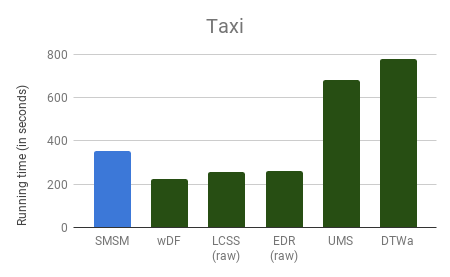
\includegraphics[width=\linewidth]{Images/running_time_CRAWDAD.png}
        \caption{}
        \label{fig:running_time_crawdad}
    \end{subfigure}
    \begin{subfigure}{0.45\textwidth}
        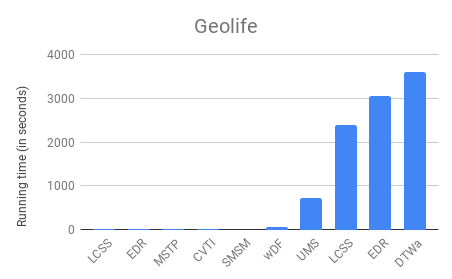
\includegraphics[width=\linewidth]{Images/running_time_Geolife.png}
        \caption{}
        \label{fig:running_time_geolife}
    \end{subfigure}\hfill % <-- added
    \begin{subfigure}[c]{0.5\textwidth}
        \centering
        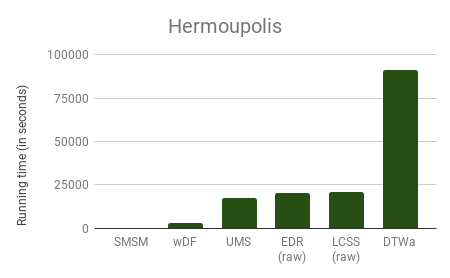
\includegraphics[width=\linewidth]{Images/running_time_Hermoupolis.png}
        \caption{}
        \label{fig:running_time_hermoupolis}
    \end{subfigure}\hfill % <-- added
    \caption{The running time of each measure in the following datasets: (a) Taxi, (b) Geolife, and (c) Hermoupolis. The running times of the similarity measures for raw trajectories are in blue, for semantic trajectories are in green, and the running time of SMSM is in yellow. }
    \label{fig:running_time_graphs}
\end{figure*}

The higher precision in the retrieval information tasks of all experiments allied with shorter running times showed SMSM as a more powerful and efficient similarity measure when the movement of the moving object is relevant.

\section{Discussion}\label{sec:discussion}

{Trajectory data can have several formats. Depending on the format and the application requirements, different trajectory analysis and mining methods will be needed, and so different similarity measures can be applied. For applications that use raw GPS data, as trajectories of taxis, buses, or cars, with the intend to detect, for instance, traffic conditions or traffic jams, the most appropriate measures are UMS and DTWa. UMS is robust for trajectories with different sampling rates or different distances between trajectory points (the case when a trajectory varies the speed in a city), because instead of using a radius around each trajectory point to find the similar trajectories in the spatial neighbourhood, it uses ellipses between every two trajectory points, and the size of the ellipses is dinamically defined based on the distance between two trajectory points. UMS is not the best measure in highly sampled trajectories, where the ellipses are very small, and in this case DTWa is  a good choice.}

{For applications that use GPS trajectories annotated only with stops or where the moves are not important, or trajectories extracted from social media data, which are more sparse and that do not have moves, the best measure is MSM. MSM is useful in applications where one is interested in finding users that visit the same places, at similar times, but where the order of the visits is not important. In tourism applications where the analyst wants to find similar tourist trajectories to either predict or to recommend the next place to be visited, MSM is not appropriate because it ignores the order. When the sequence of the visited places is important, even when the details about the moves are not, SMSM is more appropriate, because it considers the order of the stops.}

{For dealing with GPS trajectories enriched with both stops and moves, and the spatial, temporal or semantic characteristcs of both stops and moves are important, SMSM is the most appropriate measure. In a tourism application, for instance, where the tourist has a time constraint to visit a city, a sequence of visits can be recommended based on the similarity analysis of other tourists that visited the same city. SMSM is also robust in applications that focus on the most similar paths or popular routes between stops.}

{It is important to emphasize that in applications where the spatial movement of the moves is important, i.e., the raw trajectory points, SMSM can use UMS for the move similarity when trajectories have low sampling rate and DTW when trajectories have high sampling rate.}
